\documentclass[11pt]{article}
\usepackage[margin=0.8in]{geometry}\usepackage[T1]{fontenc}\usepackage{lmodern,tikz,hyperref}
\setlength{\parindent}{0pt}\setlength{\parskip}{8pt}\sloppy
\begin{document}
\begin{center}{\Large Independent conditional signed-pair review}\\1 November 2026\end{center}
Three producer declarations, three producer controls and eight reviewer controls passed fresh isolated Lean replay. A separate axiom readback covered all 14 declarations and listed only propext, Classical.choice and Quot.sound. No discrepancy was found in the abstract conditional uniqueness statement.
\begin{center}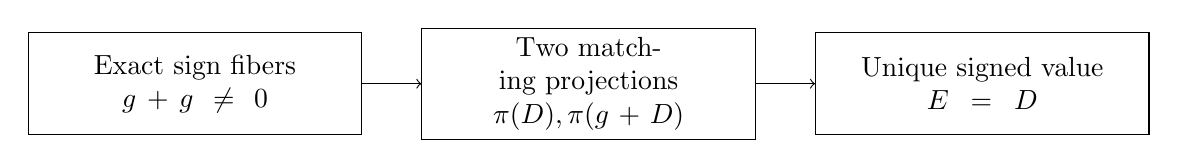
\begin{tikzpicture}[every node/.style={draw,text width=4cm,align=center,minimum height=1.3cm}]
\node (a) at (0,0) {Exact sign fibers\\$g+g\ne0$};\node (b) at (5,0) {Two matching projections\\$\pi(D),\pi(g+D)$};\node (c) at (10,0) {Unique signed value\\$E=D$};\draw[->] (a)--(b);\draw[->](b)--(c);
\end{tikzpicture}\end{center}
\textbf{Independent derivation.} Equal first projections imply $E=D$ or $E=-D$. In the opposite-sign case the neighbor equality either implies equality directly or forces $g=-g$, contradicting $g+g\ne0$. This establishes uniqueness, not existence. The prospective plan preceded proof-body inspection.

\textbf{Reviewer controls.} Actual sign-quotient functions on ZMod4 and ZMod5 have kernel-checked fibers. Eight controls cover their fiber identities, a nonzero order-two anchor ambiguity, insufficiency of one projection, neighbor separation, failure of a constant projection's fiber property, application of the main theorem, and an empty candidate set for an impossible requested coordinate. No native\_decide was used.

\textbf{Source correspondence.} The saved delta\_lift and degree-one boundary\_lift filter candidates using validity and both projection matches, returning a value only when exactly one remains. This matches the theorem's conditional uniqueness interface. The identity shortcut instead recognizes a chart coordinate pattern and checks only the anchor-neighbor projection; that coordinate recognition needs its own correctness statement.

\textbf{Projective boundary.} Raw same\_k checks cross-product equality, which accepts the zero vector against every vector. The reviewed filters reject zero supplied vectors and project\_any rejects zero output. Connecting these checks to the abstract quotient function still requires the nonzero-representative invariant, projective quotient construction and exact source fiber theorem. The anchor premise also remains a caller obligation.

\textbf{Trust and scope.} Fresh private target modules used Lean4.34.1 and retained dependency caches. The adjacent independent-product source/object snapshot was hash-bound around replay; broader Mathlib caches were reused. Inputs are private exact snapshots, not published commits. Full formal-review workflow completion, compiled Rust equivalence, geometric fiber correctness and xadd closure are not claimed.

Source anchors: source/pruned.rs lines150--181; source/walk\_impl\_uncached.rs lines51--53. Exact hashes, replay receipts, full controls and source findings accompany REVIEW.md and status.json. Full cohort scope remains 1,260; no scientific execution or measurements occurred.
\end{document}
